\chapter{数值计算}
\label{ch:numerical}

\gls*{ml}算法通常需要大量的数值计算。这通常指那些解决数学问题的算法,这样的算法使
用的方法是通过一个迭代的过程,而不是给定一个对正确解的象征性的表达式分析导出一个
公式。常见的操作包括优化(找到一个参数的值,最小化或者最大化一个函数)和解线性方
程组。当函数涉及到实数,在一个计算机上即使只是对一个数学函数求值都是困难的,它无
法用有限内存精确表示。

\section{上溢和下溢}
\label{sec:overflow_and_underflow}

在一个数字计算机上做连续的数学计算的主要困难,是我们需要用一个有限的、以 bit 位的
模式的数字来表示无限多的实数。这意味着对于几乎所有的实数,当我们在计算机中表示这
些数字时引起了一些近似误差。在多数情况下,这仅仅是舍入误差。舍入误差是有问题的,
尤其是当它经过许多操作后进一步恶化,并且,如果算法没有被设计为最小化舍入误差的累
加,它们能使理论上可行的算法在实际中失败。

一种特别严重的舍入误差的形式是\emph{\gls{underflow}}。\gls*{underflow}发生在当数
字接近 $0$ 而被舍入为 $0$ 的时候。许多函数当它们的参数为 $0$ 而不是一个小的正数时
表现出本质上的不同。例如,我们通常想要避免被 $0$ 除(当这种情况发生时有些软件环境
会产生异常,其它的会返回结果为一个占位符 \verb!not-a-number! 的值)或者取 $0$ 的
对数(这通常被当作 $-\infty$ 对待,如果它被用于更进一步的算数操作会变
成 \verb!not-a-number!)。

另一个有高度破坏性的数值误差的形式是\emph{\gls{overflow}}。\gls*{overflow}发生在
当具有大的数量级的数字被近似为 $\infty$ 或 $-\infty$ 的时候。进一步的算数计算通常
把这些无限值改为 \verb!not-a-number! 值。

一个函数必须针对\gls*{underflow}和\gls*{overflow}稳定化的函数是\gls*{softmax}函
数。\gls*{softmax}函数常常被用于预测和一个多项分布关联的概率。\gls*{softmax}函数
被定义为
\begin{equation}
  \mathrm{softmax}(\pmb{x})_i = \frac{\exp(x_i)}{\sum_{j=1}^n\exp(x_j)}
\end{equation}

考虑当所有的 $x_i$ 等于某个常数 $c$ 时会发生什么。通过分析,我们能够看到所有的输
出应该等于 $\frac{1}{n}$。从数字上看,当 $c$ 有很大的数量级时这可能不会发生。如
果 $c$ 是很小的负数,那么 $\exp(c)$ 会\gls*{underflow}。这意味着\gls*{softmax}的
分母会变成 $0$,所以最后的结果是未定义的。当 $c$ 是非常大的正数,$\exp(c)$ 会
\gls*{overflow},再一次导致整个表达式为未定义的。这两个困难都能够通过对
$\mathrm{softmax}(\pmb{z})$~——~这里 $\pmb{z} = \pmb{x} - \max_ix_i$~——~求值来解
决。通过分析,简单的代数显示,将输入\gls*{vec}加上或者减去一个标量,
$\mathrm{softmax}$ 函数的值不会被改变。对 $\max_ix_i$ 做减法导致 $\exp$ 有最大的
参数而为 $0$,这排除了\gls*{overflow}的可能。同样地,分母中至少一项值为 $1$,这
排除了分母中导致被 $0$ 除的\gls*{underflow}的可能。

还有一个小问题。分子上的\gls*{underflow}仍然能引起整个表达式求值为 $0$。这意味着
如果我们通过先运行 $\mathrm{softmax}$ 子程序然后传递其结果给 $\log$ 函数来实
现 $\log\mathrm{softmax(\pmb{x})}$ 时,我们会错误地得到
$-\infty$。相反,我们必需实现一个单独的函数,它以一个在数值上稳定的方式计
算 $\log\mathrm{softmax}$。$\log\mathrm{softmax}$ 函数能够使用我们用于稳定
化 $\mathrm{softmax}$ 函数的相同技巧来被稳定。

在这本书中,对于大部分内容,我们没有明确地详细说明所有涉及到实现不同算法的数值上
的考虑。底层库的开发者应该在实现\gls*{dl}算法时把数值问题记在心里。本书的大部分读
者可以简单地依赖已经提供稳定实现的底层库。在有些情况下,有可能实现一个新的算法并
且自动让新的实现稳定化。Theano
\citep{bergstra+al:2010-scipy-small,Bastien-2012}是一个软件包的例子,它自动检测并
稳定化许多常见的、出现在\gls*{dl}环境中的、数值上不稳定的表达式。

\section{不合理的条件作用}
\label{sec:poor_conditioning}

条件作用是指一个函数如何随着它的输入中的微小变化快速改变。那些当它们的输入被微小
扰动时快速变化的函数可能对科学计算是有问题的,这是因为在输入中的舍入误差可以导致
输入上的巨大变化。

考虑函数 $f(\pmb{x}) = \pmb{A}^{-1}\pmb{x}$。当 $\pmb{A} \in \mathbb{R}^{n
  \times n}$ 有一个\gls*{eigen-val}分解,它的\emph{\gls{cond-num}}\,是
\begin{equation}
  \max_{i,j}|\frac{\lambda_i}{\lambda_j}|
\end{equation}

这是最大和最小幅度的\gls*{eigen-val}的比率。当这个数很大时,矩阵求逆对于输入中的
误差是特别敏感的。

这个敏感性是矩阵本身的一个本质特性,不是在矩阵求逆中舍入误差的结果。当我们用真的
逆矩阵相乘时,条件不合理的矩阵放大了预先存在的误差。在实践中,这个误差会被求逆过
程自身中的误差进一步加剧。

\section{基于梯度的最优化}
\label{sec:gradient-based_optimization}

大部分\gls*{dl}算法涉及到某种优化。优化是指通过改变 $\pmb{x}$ 来最小化或者最大化
某个函数 $f(\pmb{x})$ 的任务。我们通常以最小化 $f(\pmb{x})$ 的形式表达大部分优化
问题。最大化可以通过一个最小化 $-f(\pmb{x})$ 的算法来完成。

\begin{figure}[h]
  \centering
  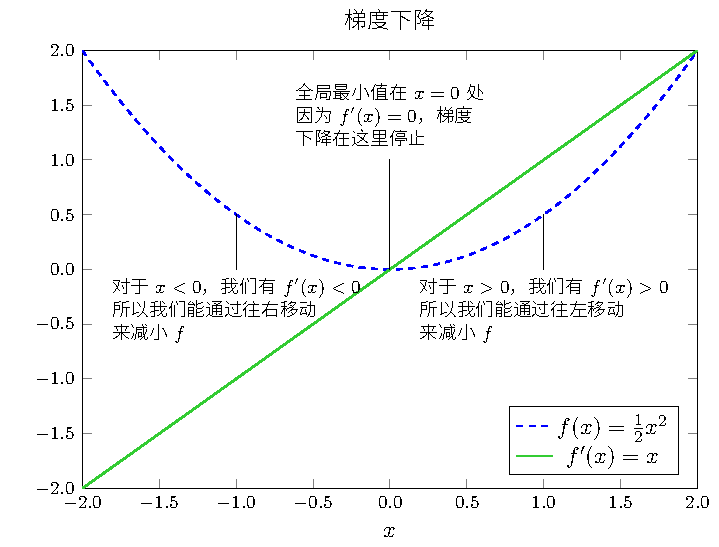
\includegraphics{gradient_descent}
  \caption{一个图例\label{fig:gradient_descent}}
\end{figure}
